% REMEMBER TO SET LANGUAGE!
\documentclass[a4paper,10pt,english]{article}
\usepackage[utf8]{inputenc}
\usepackage[english]{babel}
% Standard stuff
\usepackage{amsmath,graphicx,varioref,verbatim,amsfonts,geometry}
% colors in text
\usepackage[usenames,dvipsnames,svgnames,table]{xcolor}
% Hyper refs
\usepackage[colorlinks=false]{hyperref}

% Document formatting
\setlength{\parindent}{0mm}
\setlength{\parskip}{1.5mm}

%Color scheme for listings
\usepackage{textcomp}
\definecolor{listinggray}{gray}{0.9}
\definecolor{lbcolor}{rgb}{0.9,0.9,0.9}

%Listings configuration
\usepackage{listings}
%Hvis du bruker noe annet enn python, endre det her for å få riktig highlighting.

\lstdefinelanguage{python}
{
	morekeywords={print,abs,for,def,if,while,do,break,return,from,import,try,except,else,elif},
	sensitive=false,
	morecomment=[l]{\#}
}

\lstset{language=python,
	backgroundcolor=\color[rgb]{.95,.95,.95},
	numbers=left,xleftmargin=10pt,
	numberstyle=\tiny,stepnumber=1,numbersep=5pt,
	stringstyle=\color{red},
	basicstyle=\footnotesize \ttfamily,
	keywordstyle=\color{blue},
	commentstyle=\color{green},
	basewidth=0.60em,
	showstringspaces=false,
	captionpos=b,
	frame=single
}

\newcounter{subproject}
\renewcommand{\thesubproject}{\alph{subproject}}
\newenvironment{subproj}{
\begin{description}
\item[\refstepcounter{subproject}(\thesubproject)]
}{\end{description}}

%Lettering instead of numbering in different layers
% \renewcommand{\labelenumi}{\alph{enumi}}
\renewcommand{\thesubsection}{\alph{subsection}}

%opening
\title{FYS-MEK1110 - Mandatory assignment 2}
\author{William Dugan}

\begin{document}

\maketitle

\section{Ball on a spring}
\subsection{Free-body diagram}

\begin{figure}[h!]
        \centering 
        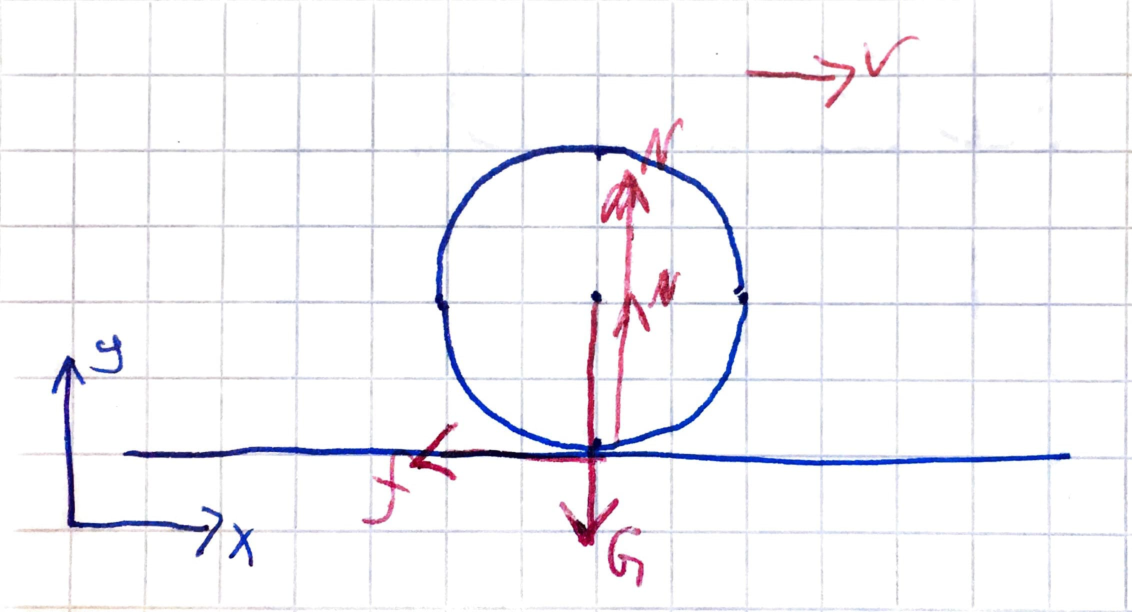
\includegraphics[scale=.35]{freebodydiagram.pdf} 
        \caption{Force due to gravity $G$ and tension in spring $T$ on ball.}
        \label{fig:forces}
\end{figure}

\subsection{Net force}
We have $\Vec{F_{net}} = \sum \Vec{F} = \Vec{G} + \Vec{T}$. Since we define our coordinate system as shown in Figure \ref{fig:forces}, we identify $G$ to be $-mg$ in the opposite direction of our y-axis. The tension in the string is given by Hooke's law and is $k * \Delta x$ in the opposite direction of our position vector. Hence
\begin{align}
    \Vec{F_{net}} 
    = \sum \Vec{F}
    = -mg\Vec{j} - k(r-L_0)\frac{\Vec{r}}{r}.
    \label{force-eq}
\end{align} 

\subsection{Component forces}
With $r = \sqrt{x^2(t)+y^2(t)}$ we get
\begin{align*}
    \Vec{F_{net}} 
    &= -mg\Vec{j} -k(\sqrt{x^2+y^2}-L_0)\frac{x\Vec{i} +         y\Vec{j}}{\sqrt{x^2+y^2}} \\
    &= \left( -k(\sqrt{x^2+y^2}-L_0) \frac{x(t)}{\sqrt{x^2+y^2}} \right)\Vec{i}
        + \left( -mg\Vec{j} - k(\sqrt{x^2+y^2}-L_0)\frac{    y(t)}{\sqrt{x^2+y^2}} \right) \Vec{j}
\end{align*}
If we split this into its separate components we get
\begin{align}
    F_x = \left[ -k\left(1-\frac{L_0}{\sqrt{x^2(t)+y^2(t)}}\right) x(t) \right] \Vec{i} \\
    F_y = \left[ -mg - k\left(1-\frac{L_0}{\sqrt{x^2(t)\y^2(t)}}\right) y(t) \right] \Vec{j}
\end{align}

\subsection{Position expressed by $\theta$}
If we were to express the position of the ball by using polar coordinates given by $\theta$ and $r$ instead of Cartesian coordinates, we would need to know the length of the spring as well. This means that the angle $\theta$ does not give a sufficient description of the balls position. 

\subsection{No movement nor acceleration}
If $\theta = 0$ and $\Vec{v} = \Vec{a} = \Vec{0}$, the ball would simply be resting at its equilibrium position. This position is given by $\Vec{r} = (0, -L_0)$.

\subsection{Expressing the acceleration}
From Newton's second law we have
\begin{align}
    \sum \Vec{F} = m \Vec{a}
\end{align}
We get the acceleration by dividing equation \ref{force-eq} by the ball's mass. This gives us
\begin{align}
    \Vec{a_{net}} 
    = \frac{\Vec{F_{net}}}{m}
    = -g\Vec{j} - \frac{k}{m}\left( 1-\frac{L_0}{r} \right) \Vec{r}.
\end{align}
The components of acceleration in x and y direction is easily found by dividing $F_x$ and $F_y$ by the ball's mass, giving us
\begin{align}
    a_x = - \frac{k}{m} \left( 1 - \frac{L_0}{\sqrt{x^2(t)+y^2(t)}} \right) x(t) \\
    a_y = -g - \frac{k}{m} \left( 1 - \frac{L_0}{\sqrt{x^2(t)+y^2(t)}} \right) y(t)
\end{align}

\subsection{Differential equation for $\Vec{a}(t)$}
We want to solve the following equations using the Euler-Cromer method
\begin{align*}
    v(t + \Delta t) &= v(t) + a(t) \Delta t \\
    r(t + \Delta t) &= r(t) + v(t) \Delta t \\
                    &= r(t) + v(t + \Delta t) \Delta t.
\end{align*}
To solve this we need the initial positions, velocities and acceleration (as well as $t(0) = t_0$). The initial velocity is $\Vec{v} = \Vec{0}$. The initial position is given by 
\begin{align*}
    r_0 = (L_0 sin(\theta_0), -L_0 cos(\theta_0)) = (sin(\pi/6), -cos(\pi/6)).
\end{align*}
We will calculate the initial acceleration at the start of our integration loop, so there is no need to perform any further calculations. 

\subsection{Numerical solution to differential equation}
\lstinputlisting{oblig2.py}

\newpage
\subsection{Results from program}
The program is set to run with $\Delta t = 0.001$s for 10s. 
\begin{figure}[h!]
        \centering 
        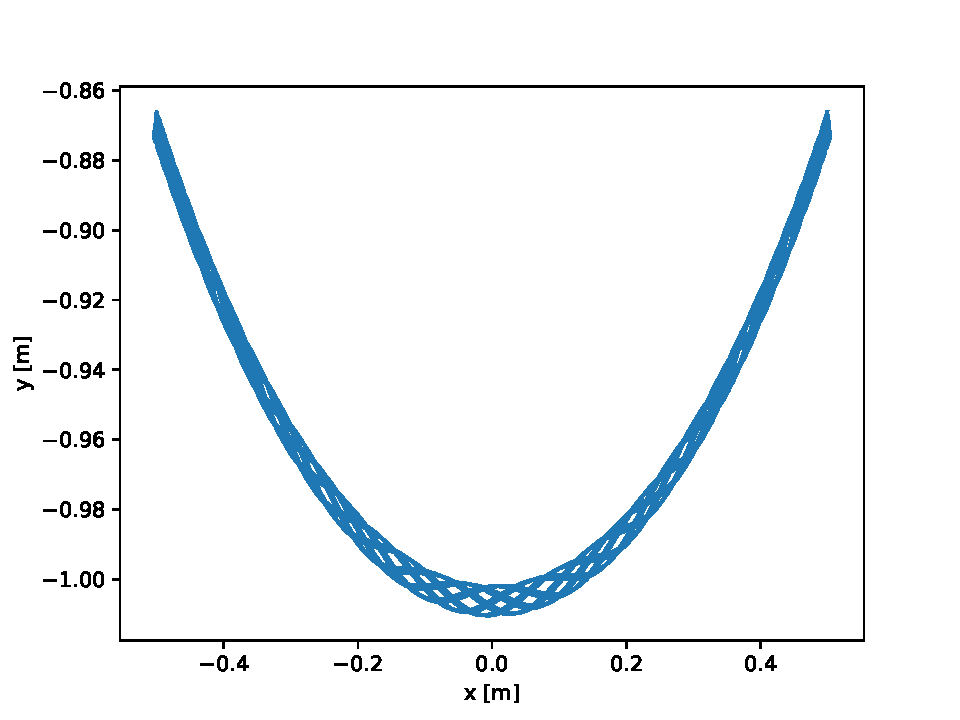
\includegraphics[scale=.7]{mainplot.pdf} 
        \caption{Plot of $x, y$ for $t\in[0, 10]$}
        \label{xy}
\end{figure}

In Figure \ref{xy} we can see that the ball oscillates in an expected manner. The movement in the $x$ direction is what we would expect from a standard pendulum on a string, but we can clearly see that it oscillates in the y-direction as well. This is what created the webbing / knitting pattern we observe. 

\subsection{Changes to $\Delta t$}
With $\Delta t = 0.01$s it seems as the time taken for a vertical oscillation decreases, giving us a tighter webbing pattern, but the motion is generally the same as before. Using $\Delta t = 0.1$s I receive an Runtime Warning: Overflow and the resulting plot is a straight line with $x,y >> 10^{200}$. I chose to not implement Euler's method as it is proven to be far less accurate when dealing with periodic motion. 

\newpage
\subsection{Changes to spring constant $k$}
\begin{figure}[h]
    \centering
    \begin{minipage}{0.5\textwidth}
        \centering
        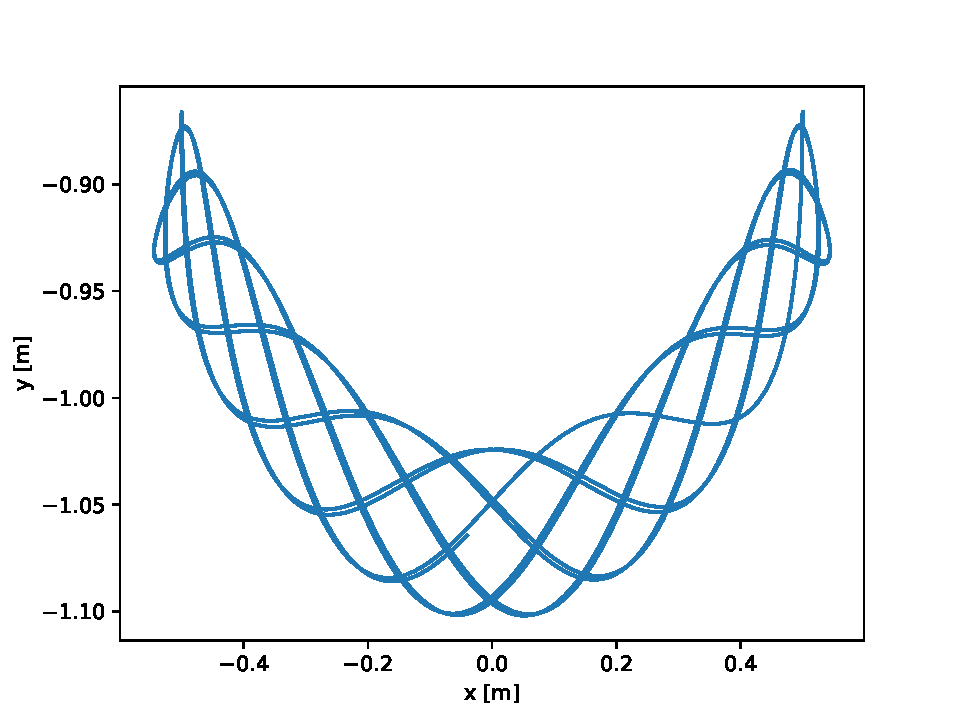
\includegraphics[width=1.05\textwidth]{k20.pdf} % first figure itself
    \end{minipage}\hfill
    \begin{minipage}{0.5\textwidth}
        \centering
        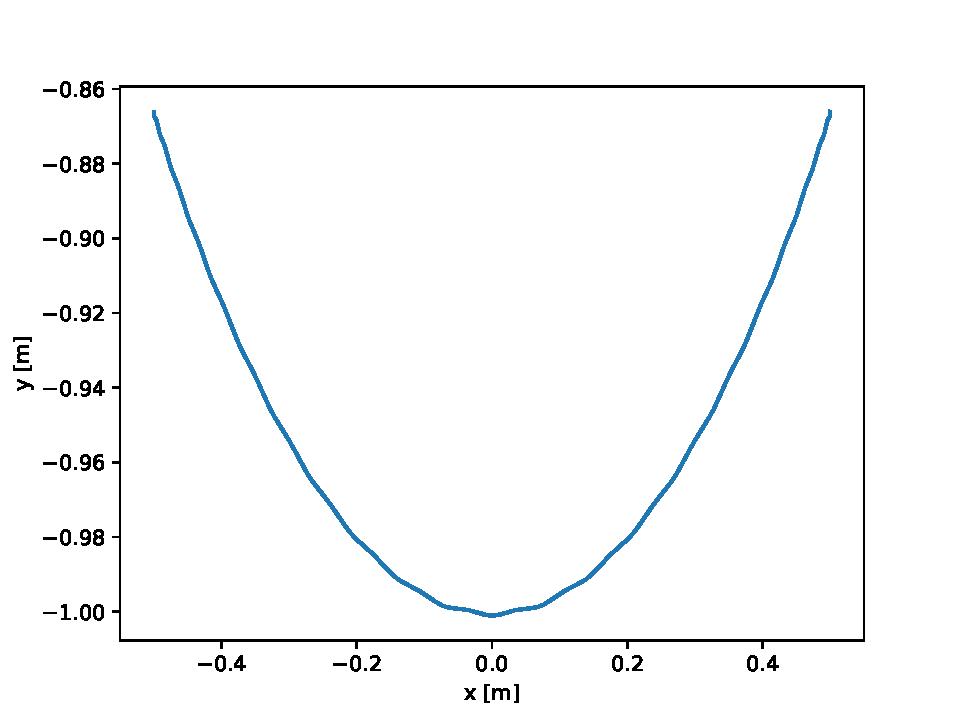
\includegraphics[width=1.05\textwidth]{k2000.pdf} % second figure itself
    \end{minipage}
    \caption{Plot of $x, y$ for $t\in[0, 10]$ with $k = 20$ and $k = 2000$ respectively.}
    \label{dt}
\end{figure}
Figure \ref{dt} shows how a stiffer spring (higher $k$) results in a motion more similar to a pendulum on a non-elastic string. When trying to run the program with $k=2*10^6$ I received another Runtime Warning: Overflow. This shows that even though our model will be closer to a non-elastic spring by simply increasing the spring constant, it lacks in efficiency and the model becomes inaccurate at some point. 

\end{document}
